\documentclass[10pt,a4paper]{scrartcl}
\usepackage[utf8]{inputenc}
\usepackage[T1]{fontenc}
\usepackage[ngerman]{babel}
\usepackage{microtype, multicol, marginnote, bera, parskip}
\usepackage{listings, amsmath, amssymb, graphicx, tikz, epic}
\usepackage{stmaryrd} %for lightning arrow
\usepackage{pstricks, pst-node, pst-tree, pdflscape}
\usepackage[babel=true]{csquotes}
\tolerance=2000
\setcounter{secnumdepth}{0}
\usepackage[inner=2.5cm,outer=2.5cm,top=1.5cm,bottom=1.5cm,includeheadfoot]{geometry}

\author{Michael Mardaus}
\title{
\includegraphics[scale=0.2]{logo_schriftzug}\\ Technische Informatik:
Abgabe 2}

\begin{document}

\maketitle


\section{Aufgabe 1}
Funktion:
$f(a,b,c)=a.b + a.c + \neg b.c + a.\neg c + b.c$\\
\subsection{a)}
\begin{tabular}{|l||l|l|l||l|}\hline
i & $a$ & $b$ & $c$ & $f(a,b,c)$ \\\hline\hline
0 & 0 & 0 & 0 & 0 \\\hline
1 & 0 & 0 & 1 & 1 \\\hline
2 & 0 & 1 & 0 & 0 \\\hline
3 & 0 & 1 & 1 & 1 \\\hline
4 & 1 & 0 & 0 & 1 \\\hline
5 & 1 & 0 & 1 & 1 \\\hline
6 & 1 & 1 & 0 & 1 \\\hline
7 & 1 & 1 & 1 & 1 \\\hline
\end{tabular} 

\paragraph{DNF}
DNF = Minterme der einschlägigen Indizes (Sum of Products)\\
$m_1 + m_3 + m_4 + m_5 + m_6 + m_7 = \neg a.\neg b.c + \neg a.b.c + a.\neg b.\neg c + a.\neg b.c + a.b.\neg c + a.b.c$

\subsection{b) Nur mit 3 NAND Gattern darstellen}
$f(a,b,c) = a + c$ (siehe Tabelle)\\
$= \neg(\neg a.\neg c) = \neg((a\uparrow a).(c\uparrow c)) = (a\uparrow a) \uparrow (c\uparrow c)$

\section{Aufgabe 2}
Beweisen oder widerlegen Sie: NOR ist assoziativ:\\
$(1 \downarrow 0) \downarrow 0 = 0 \downarrow 0 = 1$\\
$1 \downarrow (0 \downarrow 0) = 1 \downarrow 1 = 0 \quad \lightning$\\
NOR ist nicht assoziativ.

\section{Aufgabe 3}
\subsection{a) Tabelle}
\begin{tabular}{|l||l|l|l||l|}\hline
i & $s_1$ & $s_2$ & $s_3$ & $f(s_1,s_2,s_3)$ \\\hline\hline
0 & 0 & 0 & 0 & 0 \\\hline
1 & 0 & 0 & 1 & 0 \\\hline
2 & 0 & 1 & 0 & 0 \\\hline
3 & 0 & 1 & 1 & 1 \\\hline
4 & 1 & 0 & 0 & 0 \\\hline
5 & 1 & 0 & 1 & 1 \\\hline
6 & 1 & 1 & 0 & 0 \\\hline
7 & 1 & 1 & 1 & 1 \\\hline
\end{tabular}
\hspace{2cm}
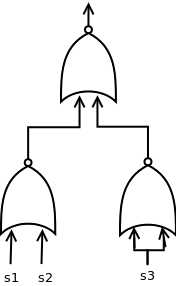
\includegraphics[width=2cm]{2-3-b.png}

\subsection{b) KNF}
KNF = Maxterme (=$\neg$ Minterme) der nullschlägigen Indizes (Product of Sums)\\
$M_0 . M_1 . M_2 . M_4 . M_6 = (s_1+s_2+s_3) . (s_1+s_2+\neg s_3) . (s_1+\neg s_2+s_3) . (\neg s_1+s_2+s_3) . (\neg s_1+\neg s_2+s_3)$\\
$= ((s_3.\neg s_3)+s_1+s_2) . (\neg s_1+s_2+s_3) . ((s_1.\neg s_1)+\neg s_2+s_3) $\\
$= (s_1+s_2) . (\neg s_1+s_2+s_3) . (\neg s_2+s_3)$\\
...$(s_1 \downarrow s_2) \downarrow (s_3 \downarrow s_3)$


\section{Aufgabe 4}

\begin{tabular}{|l||l|l|l|l||l|l|l|l|}\hline
i & $a$ & $b$ & $c$ & $d$ & \multicolumn{4}{|c|}{$f(a,b,c,d)$} \\\hline\hline
0 & 0 & 0 & 0 & 0 &    0 & 0 & 0 & 1 \\\hline
1 & 0 & 0 & 0 & 1 &    0 & 0 & 1 & 0 \\\hline
2 & 0 & 0 & 1 & 0 &    0 & 0 & 1 & 1 \\\hline
3 & 0 & 0 & 1 & 1 &    0 & 1 & 0 & 0 \\\hline
4 & 0 & 1 & 0 & 0 &    0 & 1 & 0 & 1 \\\hline
5 & 0 & 1 & 0 & 1 &    0 & 1 & 1 & 0 \\\hline
6 & 0 & 1 & 1 & 0 &    0 & 1 & 1 & 1 \\\hline
7 & 0 & 1 & 1 & 1 &    1 & 0 & 0 & 0 \\\hline
8 & 1 & 0 & 0 & 0 &    1 & 0 & 0 & 1 \\\hline
9 & 1 & 0 & 0 & 1 &    1 & 0 & 1 & 0 \\\hline
10 & 1 & 0 & 1 & 0 &   1 & 0 & 1 & 1 \\\hline
11 & 1 & 0 & 1 & 1 &   1 & 1 & 0 & 0 \\\hline
12 & 1 & 1 & 0 & 0 &   1 & 1 & 0 & 1 \\\hline
13 & 1 & 1 & 0 & 1 &   1 & 1 & 1 & 0 \\\hline
14 & 1 & 1 & 1 & 0 &   1 & 1 & 1 & 1 \\\hline
15 & 1 & 1 & 1 & 1 &   0 & 0 & 0 & 0 \\\hline
\end{tabular}
\hspace{1cm}
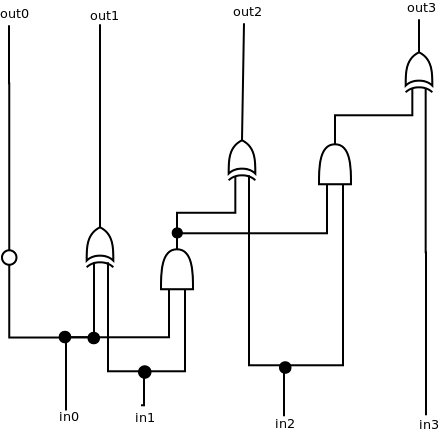
\includegraphics[width=6cm]{2-4.png}



\end{document}